En este capítulo vamos a dar una introducción a las bases de datos tipo NoSQL, veremos los principales usos de estas así como comparativas con bases de datos de tipo SQL.

Terminaremos este capítulo viendo las características más relevantes de la base de datos MongoDB, la que utilizaremos en nuestro trabajo para dar una propuesta de un motor difuso para consultas sobre esta plataforma.

\section{Introducción}

NoSQL - \texttt{Not only SQL} - la primera ocurrencia del término  según \cite{chalmerthesis} data de 1998 cuando Carlo Strozzi lo utiliza para denominar a la base de datos que había creado, una base de datos \textit{open-source} relacional, \cite{strozzidb}, pero que no proveía de una interfaz SQL. 
En 2009 Eric Evan retoma el término en unas conferencia sobre bases de datos \textit{open-source}.

A pesar de estas fechas y momentos puntuales, lo cierto es que las bases de datos clave-valor, por ejemplo, ahora consideradas NoSQL, existen desde mucho antes, por lo que es difícil establecer el momento preciso en que surge el concepto de NoSQL. 

Hay muchas diferencias entre las base de datos NoSQL y los SGBDRs (Sistemas de Gestión de Bases de Datos Relacionales), veremos más adelante algunas de ellas, pero podemos destacar dos: no usan el lenguaje SQL como lenguaje principal de consulta y no garantizan completamente ACID (atomicidad, consistencia, aislamiento y durabilidad). Veamos que significan estos términos:

\begin{itemize}
    \item Atomicidad: Las transacciones son completas, esto es, si uan operación comprende más de un paso, o se realizan todos o no se realiza ninguno.
    \item Consistencia: Este término se refiere a la integridad de los datos, las operaciones llevan la base de datos desde un estado válido a otro estado válido
    \item Aislamiento: Este término hace referencia a la independencia de operaciones. Una operación no puede afectar a otra.
    \item Durabilidad: Esta propiedad asegura que una vez realizada una operación, perdurará en el tiempo aún si el sistema se falla.
\end{itemize}

La utilidad de este tipo de bases de datos se ha incrementado recientemente por la necesidad de incrementar el almacenamiento de datos. Son las principales bases de datos para las técnicas de \textit{Big Data} y el manejo de grandes cantidades de datos. Suelen escalar bien horizontalmente y permiten el almacenamientos de distintas formas. Veremos los tipos de bases de datos NoSQL y algunos ejemplos en la siguiente sección.

\subsection{Teorema de CAP}
En \cite{captheorem} se introduce el \textbf{teorema de CAP} que establece que es imposible para un sistema computacional distribuido ofrecer simultáneamente las siguientes tres garantías:

\textbf{Consistencia}: La información tiene que ser la misma para una operación independientemente del nodo en el que se haga.

\textbf{Disponibilidad}: La información tiene que estar accesible para todos los clientes independientemente de que algún nodo no esté disponible.

\textbf{Tolerancia a particiones}: El sistema tiene que seguir disponible aunque existan problemas de comunicación entre algunos nodos o alguno de ellos se encuentre caído.

En base a éste teorema, en la siguiente figura podemos ver como se clasifican algunas de las bases de datos más utilizadas, atendiendo a las dos características que éstas garantizan:

\begin{figure}[h]
  \centering
  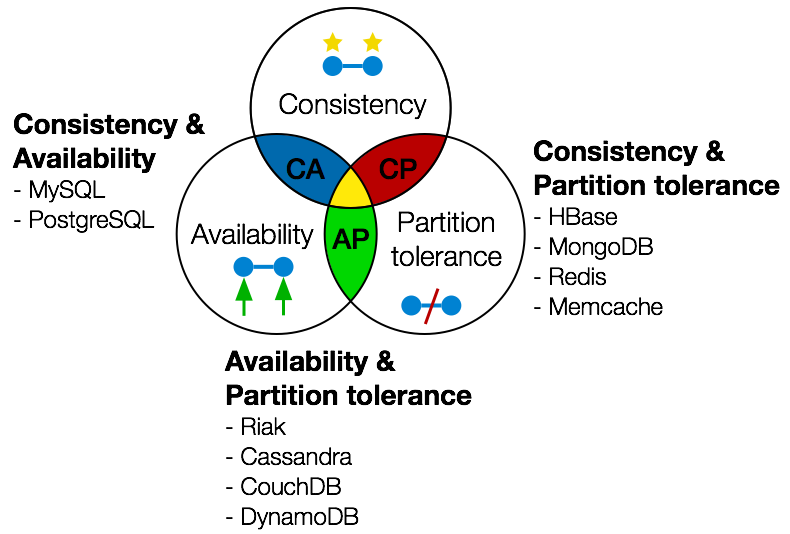
\includegraphics[width=0.9\textwidth]{gfx/CAPTheorem.png}
  \caption{Clasificación de bases de datos mediante el teorema de CAP.}
\end{figure}

\section{Tipos de bases de datos NoSQL}

En esta sección vamos a caracterizar las bases de datos NoSQL según la forma en la que almacenan los datos. Podemos clasificar la mayoría de bases de datos NoSQL en alguna de las siguientes 4 categorías, como se describe en la propia documentación de MongoDB \cite{mongoclassification}.

\begin{itemize}
    \item \texttt{Almacenamiento clave-valor}: Son grandes tablas que almacenan la información en forma de clave-valor. Las bases de datos de este tipo más populares son: RedisDB, Riak y Voldemort.
    \item \texttt{Almacenamiento basado en documentos}: Es este tipo de bases de datos, los datos se almacenan en forma de documentos. El concepto de documento depende de la definición de la base de datos, normalmente son grandes conjuntos de claves-valor codificados o encapsulados como un tipo de documento. En esta categoría, MongoDB es el más popular y más usado, pero existen otros como CouchDB.
    \item \texttt{Almacenamiento basado en grafos}: Estas bases de datos almacenan relaciones en forma de grafos. Algunas de las bases de datos más populares son: Neo4j y FlockDB.
    \item \texttt{Almacenamiento en columnas}: En este tipo de bases de datos, se almacenan columnas en lugar de filas como en el resto de tipos. Está optimizado para grandes volúmenes de datos. Las bases de datos más populares de este tipo son: Cassandra y HBase. 
\end{itemize}

En el artículo \cite{nosqlcomparativas}, puede verse una comparativa entre distintas bases de datos NoSQL sobre lenguaje en el que están escritas, ternologías que utilizan, tipo de base de datos, etc.

\section{Comparativa NoSQL con SGBDR}

En esta sección vamos a realizar una comparativa entre las bases de datos SQL y NoSQL.

En primer lugar, además de las dos diferencias comentadas anteriormente, es de destacar, que las bases de datos NoSQL son libres de esquema, esto es, que no necesitan una planificación antes de empezar a almacenar datos a nivel de relaciones, tablas, etc. Los datos almacenados son independientes entre ellos y pueden ser totalmente distintos. Esto aporta un gran valor en el sentido de adaptabilidad a nuevos cambios.

\subsection{Sistemas de Gestión de Bases de Datos Relacionales}

Vamos a dar algunas características que caracterizan a Sistemas de Gestión de Bases de Datos Relacionales (SGBDR), para comenzar veremos algunos de las características favorables de este tipo de base de datos:

\begin{itemize}
    \item Mayor soporte y herramientas debido a su largo recorrido en el mercado.
    \item Permiten combinar diferentes tablas eficientemente para obtener información relacionada.
    \item Los datos siguen una estructura predefinida en los esquemas.
    \item Proporcionan atomicidad en las operaciones y transaccionalidad entre tablas, esto evita que se queden datos inconsistentes si hay un error en cualquier punto de una operación.
\end{itemize}

Por contra:

\begin{itemize}
    \item No son flexibles, en el sentido de que los datos tienen que seguir el esquema definido y tienen que estar correctamente validados.
    \item Incremento del procesamiento con el incremento de la complejidad en las relaciones.
    \item Dificultad para escalar, habitualmente necesitan de ampliación de hardware costoso.
\end{itemize}

\subsection{Bases de Datos NoSQL}

Una de las principales características que tendría el conjunto de bases de datos NoSQL, es que proporcionan una manera alternativa de almacenar la información y muy diversa por los tipos que comentamos anteriormente, por tanto, ya nos proporcionan una cierta ventaja de flexibilidad que no tenemos con los sistemas SGBDR tradicionales. Veamos ahora algunas características favorables que poseen las bases de datos NoSQL:

\begin{itemize}
    \item Escalabilidad. En general, tienen buen escalamiento horizontal.
    \item Soporte para modelos flexibles, libres de esquemas, tipos y validaciones.
    \item Optimizadas para grandes volúmenes de datos.
    \item Necesita de pocos recursos para su funcionamiento.
\end{itemize}

Por contra:

\begin{itemize}
    \item No todas garantizas atomicidad y consistencia en los datos.
    \item Falta de estandarización. No existe un estándar para estas bases de datos como si lo hay para las de tipo SQL.
    \item Falta de herramientas de gestión. Muchas de ellas solo son accesibles por consola.
\end{itemize}

\section{MongoDB}

En esta sección vamos a centrarnos en la base de datos NoSQL más popular hasta el momento, MongoDB es una base de datos orientada a documentos muy usada para técnicas de Big Data. Toda esta sección está extraida de la documentación oficial de MongoDB \cite{mongodb}.

Las principales características son:

\begin{itemize}
    \item MongoDB es una base de datos \textit{open source}, escrita en C++, lo que hace favorece su rapidez y le proporciona un buen rendimiento.
    \item Es una base de datos distribuida en su núcleo, por lo que es escala horizontalmente de forma fácil, permite la distribución geográfica y una alta disponibilidad.
    \item Almacenamiento de modelo de datos flexibles. Basada en documentos en forma de JSON, permite indexación y operaciones de agregación.
    \item Garantiza transacciones ACID (atomicidad, consistencia, aislamiento y durabilidad) en multidocumentos. Esta reciente característica ha sido integrada en la versión 4.0 de MongoDB.
\end{itemize}

\subsection{Modelo de datos}\label{datamodelmongo}

MongoDB nos provee de un modelo de datos flexible, esto nos permite almacenar desde un documento simple de parejas clave-valor, hasta un documento con subdocumentos embebidos y/o arrays complejos a varios niveles de profundidad.

Posee una sintaxis para realizar consultas muy variada, nos permite hacer consultas simples, con un lenguaje muy descriptivo, sofisticados \textit{pipeline} para consulta, transformación y explotación de datos, búsquedas facetadas, etc.

Mongo almacena los datos en formato BSON \cite{bsonspec} que es una extensión de los objetos nativos de JavaScript (JSON) a los que añade algunos tipos de datos extra. Estos tipos de datos, se asemejan a los objetos que encontramos en los distintos lenguajes de programación, lo que hace que se produzca una rápida adaptación y una fácil integración con el modelo de datos de MongoDB.

Una de las principales diferencias con las bases de datos relacionales a la hora de modelizar es que mientras que en las bases de datos relaciones es habitual crear distintas tablas para trabajar mediante JOINs, en MongoDB es habitual tener todos los datos necesarios para un registro en un mismo documento, lo que reduce la complejidad de tener que realizar JOINs entre tablas y ayuda a la mejora de las consultas.

\subsection{Tipos de consultas}

MongoDB tiene distintos métodos para la consulta y explotación de los datos almacenados:

\begin{itemize}
    \item Clave-valor: Búsquedas simples en cualquier campo del documento.
    \item Rangos: Es posible utilizar los operadores de desigualdades (mayor que, menor que...) para hacer búsquedas por rango y obtener un subconjunto de documentos que satisfagan las condiciones.
    \item Búsquedas Geoespaciales: Devuelven resultados basados en proximidad a ciertos criterios.
    \item Búsquedas de resutlados en un orden relevante, o en búsquedas facetadas. Es posible utilizar operadores lógicos (and, or...), agrupar, contar resultados, etc.
    \item Operador de agregación: Permite hacer consultas y transformaciones de los datos almacenados. Provee una interfaz completa de operadores dedicados (operaciones lógicas, desigualdades, proyecciones...). En este trabajo, veremos la implementación de consultas de bases de conjuntos difusos sobre este operador de agregación.
    \item JOINs y grafos: con el operador \textit{lookup} podemos hacer JOIN entre colecciones, y con el operador \textit{graphLookup} mongo provee una forma nativa de procesar grafos, árboles y estructuras jerárquicas.
\end{itemize}


\subsection{Indexación}

Según se define en la propia documentación de MongoDB \cite{mongodb}, <<\textit{la indexación es un mecanismo crucial para la optimización del rendimiento y escalabilidad del sistema mientras provee un acceso flexible a tus datos}>>. Mongo permite la indexación en cualquier campo del documento, incluso en los campos de un array.

Mongo provee la facilidad para crear índices compuestos, únicos, array, índices geoespaciales, hash y texto.

Además, la intersección de índices permite a MongoDB usar más de un índice para la optimización de las consultas.

\subsection{Agregación}

Una de las características más importante de MongoDB a la hora de explotar y transformar datos son las agregaciones. Esta base de datos nos provee dos formas de realizarla, mediante \textit{pipeline}    y mediante \textit{map-reduce}.

\subsubsection{Map-Reduce}\label{mapreduce}

Map-Reduce es un modelo de programación general muy utilizado para trabajar con grandes volúmenes de datos y poder introducir paralelismo. MongoDB provee un comando para utilizarlo directamente sobre la base de datos de forma nativa.

El modelo map-reduce, consiste en generar un subconjunto de documentos útiles preprocesando un conjunto más amplio previamente y agrupando en una última etapa.

\subsubsection{Pipeline}\label{pipeline}

La segunda forma para realizar el operador de agregación es mediante el framework \textit{pipeline}. Con este comando los documentos son procesados mediante una secuencia ordenada de etapas para producir un subconjunto de documentos. Con esta opción, una consulta normal sobre una colección se haría sobre una etapa \textit{match} de la tubería de agregación.

Las etapas permitidas para este operador se pueden encontrar en la \href{https://docs.mongodb.com/manual/reference/operator/aggregation-pipeline/}{documentación del operador}. En este trabajo, se da una ampliación de los operadores que se pueden utilizar en las etapas de \textit{match} y \textit{projection}.

La etapa \textbf{match}, como se describe en su propia documentación, sirve para filtrar los documentos que van a pasar a la siguiente etapa. Selecciona aquellos que cumplan ciertas condiciones descritas mediante los operadores permitidos para esta etapa que pueden verse \href{https://docs.mongodb.com/manual/reference/operator/query/}{aquí}. Los operadores que hemos extendido para trabajar con datos difusos son:

\begin{itemize}
    \item \textbf{\$eq}: selecciona los documentos cuyo valor coincida con el especificado.
    \item \textbf{\$gt}: selecciona los documentos cuyo valor sea mayor que el especificado.
    \item \textbf{\$gte}: selecciona los documentos cuyo valor sea mayor o igual que el especificado.
    \item \textbf{\$lt}: selecciona los documentos cuyo valor sea menor que el especificado.
    \item \textbf{\$lte}: selecciona los documentos cuyo valor sea menor o igual que el especificado.
\end{itemize}

La etapa \textbf{projection} sirve para filtrar los campos de los documentos resultantes. Nos permite tanto eliminar campos del propio documento, como proyectar campos nuevos. En esta parte nos hemos centrado en ampliar la posibilidad de proyectar el grado de cumplimiento para los campos difusos.

En el capítulo \ref{propuesta} veremos estos operadores y la propuesta realizada para ampliar estas etapas.
